

Un túnel de viento es una herramienta que puede tener dos fines hoy en día, ya sea para un uso recreativo o para propósito científico.
Como uso científico se utiliza para observar los efectos del movimiento de aire al rededor de objetos sólidos, como también para la calibración de anemómetros, entre otros usos.

Los túneles de viento se pueden clasificar en túneles abiertos o cerrados y a su vez pueden ser verticales u horizontales (Figuras: \ref{fig:tunelRec} y \ref{fig:abierto})


\begin{figure}[htb]
	\centering
	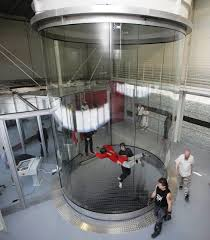
\includegraphics[scale=0.8]{tvert1.jpg}
	\captionof{figure}{Tunel uso recreativo}
	\label{fig:tunelRec}
\end{figure}

\begin{figure}[htbp]
    \centering
    \subfigure[Túnel tipo cerrado]{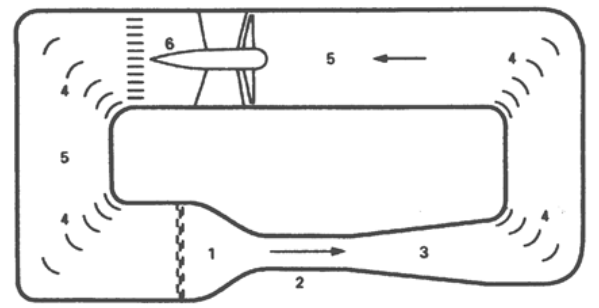
\includegraphics[width=60mm]{tunel_cerrado.png}}
    \subfigure[Túnel tipo abierto]{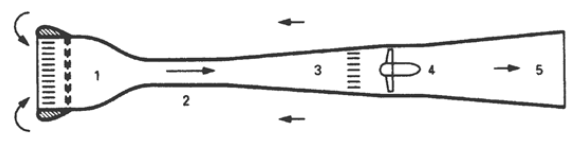
\includegraphics[width=80mm]{tunel_abierto.png}}
    \caption{Clasificación túneles} \label{fig:abierto}
    \end{figure}


\subsection{Historia del Túnel UNPSJB}


\footnote{\url{http://www.ing.unp.edu.ar/mecanica/Paginas/Tunel.htm}} 
	El túnel aerodinámico del Laboratorio de Mecánica de Fluidos (\textbf{LMF}) de la Facultad de Ingeniería de la Universidad Nacional de la Patagonia San Juan Bosco (\textbf{UNPSJB}) es un circuito abierto (tipo Eiffel) con cámara de ensayos cerrada. Puede clasificarse como un túnel “pequeño de baja velocidad”, con una longitud total de 11 $m$, una velocidad máxima de 18 $m/s$ y una cámara de ensayos con un área de 0,8 $m^2$.
	
	\begin{figure}[htb]
		\centering
		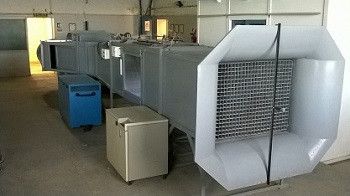
\includegraphics[scale=0.9]{tunel_unpsjb.JPG}
		\captionof{figure}{Tunel UNPSJB}
		\label{fig:tunelUni}
	\end{figure}
	
	La entrada del túnel cuenta con canalizadores, comúnmente denominados "panal de abejas", que favorecen la formación de un flujo uniforme y homogéneo propiciando mejores resultados en los experimentos.
	
	La cámara de ensayos es vidriada para poder observar con claridad el flujo y está incorporada en un módulo extraíble del túnel, lo cual permite fácil acceso para el armado de los distintos objetos a ensayar.
	
	Los distintos ensayos que se realizan en el túnel son:
	\begin{itemize}
		\item  Determinación de coeficientes de resistencia y sustentación de distintos cuerpos y perfiles aerodinámicos. 
		\item Determinación de distribución de presiones a través de diferentes objetos como perfiles aerodinámicos, edificios, puentes, automóviles, etc.
		\item Visualización con humo del flujo a través de distintos obstáculos.
		\item Estudio del comportamiento dinámico de generadores eólicos. 
		\item Calibración de anemómetros.
	\end{itemize}

	\subsubsection{Motor y Variador de velocidad}
		\begin{tcolorbox}[colback=blue!5!white,colframe=blue!75!black,title=Variador de velocidad]
			Es utilizado para controlar la velocidad de giro de un motor. Para regular las revoluciones, se debe tener en cuenta las características del motor, ya que este tiene  una  curva  propia  de  funcionamiento.  Un  variador  es  capaz  de  generar elementos  control  de  aceleración,  frenado,  seguridad,  control  del  torque  y operaciones que mejoran la eficiencia energética.\end{tcolorbox}	

		
El motor que se utiliza para hacer funcionar el ventilador corresponde a la marca \textbf{AEG}, de 30 kW de potencia\cite{barila1993desarrollo}. Mientras que el variador de velocidad, es de la marca \textbf{Long Shenq}.

El variador cuyo modelo es \textbf{LS650-4045} para una potencia de 45kW con salida trifásica es capaz de ser controlado por entradas de corriente, tensión, PID interno, potenciómetro o de forma manual con botones en su panel frontal.


\begin{figure}[htb]
	\centering
	\subfigure[Motor y ventilador durante la construcción del túnel]{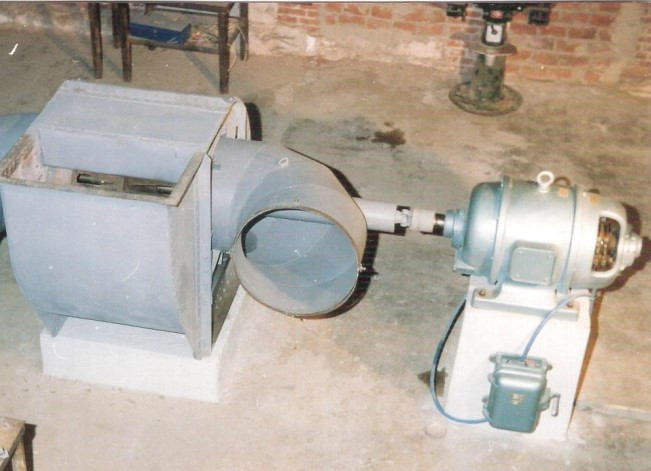
\includegraphics[height=7cm]{motor.jpg}}\label{fig:motorr}
	\hfill
	\subfigure[Variador de velocidad LS650]{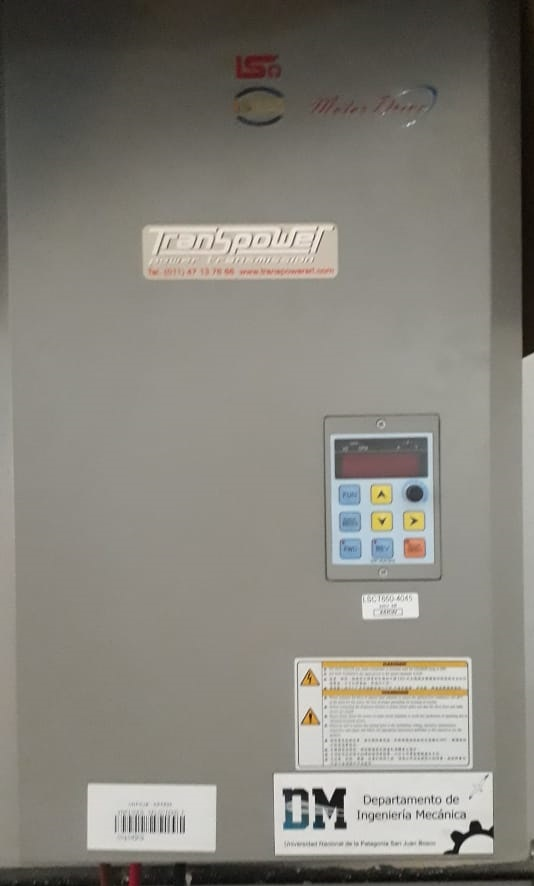
\includegraphics[height=7cm]{LS650.jpg}}\label{fig:LS650}
	\caption{Motor y variador de velocidad} 
	
\end{figure}



		
	\subsubsection{Instrumentación utilizada}
	Los instrumentos normalmente utilizados en conjunto con el túnel del viento, que están calibrados y certificados por el INTI son:
\begin{itemize}
	\item AXD 650 \textbf{ALNOR} 
		\subitem Instrumento micromanómetro utilizado para medir la diferencia de presión.
	\item Testo 435 \textbf{TESTO}
	\subitem Instrumento multifunción utilizado para medir la temperatura, humedad y presión atmosférica. Este mismo elemento puede ser utilizado para medir la velocidad del aire.
	
\end{itemize}	   		
		
\begin{figure}[htbp]
	\centering
	\subfigure[AXD 650]{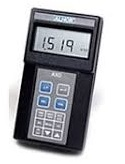
\includegraphics[width=40mm]{axd.jpg}}
	\subfigure[testo 435]{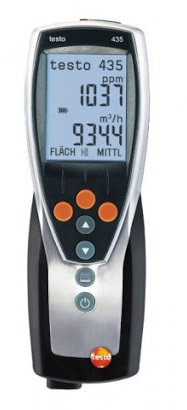
\includegraphics[scale=0.5]{testo.jpg}}
	\caption{Instrumentos calibrados} \label{fig:instr}
\end{figure}		
		
		
		\newpage